% ============================================
% 树状结构模板 (Tree Structure Templates)
% 适用：二叉树、目录树、组织架构图
% ============================================

% --------------------------------------------
% 二叉树
% --------------------------------------------
\begin{figure}[H]
  \centering
  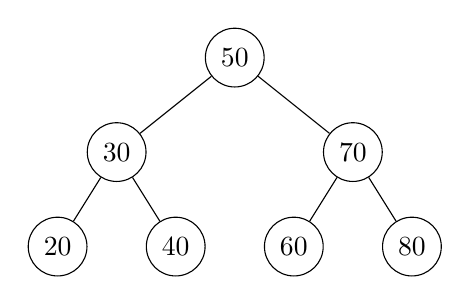
\begin{tikzpicture}[
    level distance=1.2cm,
    level 1/.style={sibling distance=3cm},
    level 2/.style={sibling distance=1.5cm},
    every node/.style={circle, draw, minimum size=0.7cm}
  ]
    \node {50}
      child {node {30}
        child {node {20}}
        child {node {40}}
      }
      child {node {70}
        child {node {60}}
        child {node {80}}
      };
  \end{tikzpicture}
  \caption{二叉搜索树示例}
  \label{fig:binary_tree}
\end{figure}

% --------------------------------------------
% 水平目录树（从左到右展开）
% --------------------------------------------
\begin{figure}[H]
  \centering
  \begin{tikzpicture}[
    grow=right,
    level distance=3cm,
    level 1/.style={sibling distance=2.5cm},
    level 2/.style={sibling distance=1.2cm},
    every node/.style={draw, rectangle, rounded corners=2pt, 
                       minimum width=1.8cm, minimum height=0.6cm, font=\small},
    edge from parent/.style={draw, ->, thick}
  ]
    \node {项目根目录}
      child {node {src/}
        child {node {main.c}}
        child {node {utils.c}}
        child {node {config.h}}
      }
      child {node {docs/}
        child {node {README}}
        child {node {API文档}}
      }
      child {node {tests/}
        child {node {test\_main}}
      };
  \end{tikzpicture}
  \caption{项目目录结构树}
  \label{fig:directory_tree}
\end{figure}

% --------------------------------------------
% 垂直层次图（组织架构，自上而下）
% --------------------------------------------
\begin{figure}[H]
  \centering
  \begin{tikzpicture}[
    level distance=1.5cm,
    level 1/.style={sibling distance=5cm},
    level 2/.style={sibling distance=2.2cm},
    every node/.style={draw, rectangle, rounded corners, 
                       minimum width=1.5cm, minimum height=0.7cm,
                       align=center, font=\small},
    edge from parent/.style={draw, thick}
  ]
    \node {总经理}
      child {node {技术部}
        child {node {开发组}}
        child {node {测试组}}
      }
      child {node {市场部}
        child {node {销售组}}
        child {node {推广组}}
      }
      child {node {行政部}
        child {node {人事}}
        child {node {财务}}
      };
  \end{tikzpicture}
  \caption{组织架构层次图}
  \label{fig:org_hierarchy}
\end{figure}
